\section{习题}
\label{sec:ch07-exercises}
% ============================================================================

这一章最容易“看懂却没真正会用”的地方，
就在于它不断跨越三种语言：
复解析语言里我们看见的是 $\Gamma_0(N)\backslash\HH^*$ 与 $j$-函数；
代数几何语言里我们看见的是方程、函数域、除子与对应；
数论语言里我们又关心 $\Q$-有理点、判别式与模 $p$ 约化。
如果只停留在概念介绍，
这三层语言很容易彼此脱节。

\textbf{我们遇到了什么问题？}
一方面，模多项式与模解释听起来都很抽象；
另一方面，Hecke 对应、整模型、好约化这些概念又都带有强烈的几何色彩。
若不亲手算几个例子，
读者往往会分不清哪些结论是“理论上存在”，哪些对象又真能落成具体方程与具体计数。

\textbf{核心思想是什么？}
所以本节习题的设计非常刻意：
先用 $\Phi_2$ 把“模曲线是代数方程”这句话落成显式公式；
再用 $X_0(11)$ 与 $T_p$ 的计数把“模解释”落成具体点集；
最后用判别式、N\'eron $n$-gon 与遗忘映射的次数，
把“整数模型”和“函子性”也拉回到可以直接计算的层面。

\textbf{引入之后能得到什么？}
做完这几题后，
你应该会真正相信三件事：
第一，模曲线确实可以写成整系数代数方程；
第二，Hecke 算子确实来自有限对应而不是偶然公式；
第三，整模型与约化并不是额外装饰，
而是把模曲线送进算术世界的必要步骤。

\begin{figure}[ht]
\centering
\begin{tikzpicture}[>=Stealth, font=\small, node distance=1.25cm]
  \node[draw, rounded corners, fill=blue!8, minimum width=5.4cm, minimum height=0.9cm] (a) {习题 1：模多项式与代数关系};
  \node[draw, rounded corners, fill=green!8, below=of a, minimum width=5.4cm, minimum height=0.9cm] (b) {习题 2--3：$X_0(11)$ 与 Hecke 对应的计数};
  \node[draw, rounded corners, fill=orange!10, below=of b, minimum width=5.4cm, minimum height=0.9cm] (c) {习题 4--5：判别式、好约化与 N\'eron $n$-gon};
  \node[draw, rounded corners, fill=purple!10, below=of c, minimum width=5.4cm, minimum height=0.9cm] (d) {习题 6：模解释的函子性与次数};
  \draw[->, thick] (a) -- (b);
  \draw[->, thick] (b) -- (c);
  \draw[->, thick] (c) -- (d);
\end{tikzpicture}
\caption{本章习题把主线重新走一遍：先从模多项式得到显式方程，再把 Hecke 对应、判别式与模解释的函子性落到可以手算的例子上。}
\label{fig:ch07-exercises}
\end{figure}


\begin{exercise}
\label{ex:ch07-phi2}
写出
\[
\begin{aligned}
\Phi_2(X,Y)=&\ X^3+Y^3-X^2Y^2+1488(X^2Y+XY^2)\\
&-162000(X^2+Y^2)+40773375XY\\
&+8748000000(X+Y)-157464000000000,
\end{aligned}
\]
并验证：若 $j=j(\tau)$，$j_2=j(2\tau)$，则 $\Phi_2(j,j_2)=0$。
解释为何成立，不要求逐项展开计算。
\end{exercise}

\begin{proof}[解答]
这件事成立的根本原因不是巧合的代数恒等式，
而是 \cref{thm:ch07-modular-polynomial} 的定义。
按定义，$\Phi_2(X,Y)$ 是把所有次数 $2$ 的循环同源关系编码进一个整系数多项式后的结果。
对格
\[
  \Lambda_\tau=\Z+\tau\Z,
  \qquad
  \Lambda_{2\tau}=\Z+2\tau\Z,
\]
自然包含
\[
  \Lambda_{2\tau}\subset \Lambda_\tau
\]
的指数正好是 $2$，
所以复环面之间有一条次数为 $2$ 的循环同源
\[
  \C/\Lambda_{2\tau}\longrightarrow \C/\Lambda_\tau.
\]
因此对应的两个 $j$-不变量 $j(2\tau)$ 与 $j(\tau)$ 必满足“存在 $2$-同源”的代数关系，
也就是
\[
  \Phi_2\bigl(j(\tau),j(2\tau)\bigr)=0.
\]

若从第\ref{sec:ch07-modular-curves-over-q}节的乘积定义来看，
$\Phi_2(X,j(\tau))$ 就是一个以所有 $j(2\gamma\tau)$ 为根的首一多项式。
其中 $\gamma=1$ 这一项已经给出根 $X=j(2\tau)$，
所以把 $X$ 取成 $j(2\tau)$ 时必然为零。
这正是所要求说明的内容。
\end{proof}

\begin{exercise}
\label{ex:ch07-x011-integral-points}
在模型
\[
  X_0(11): y^2+y=x^3-x^2-10x-20
\]
上，找出所有满足 $x,y\in\Z$ 且 $|x|\le 5$ 的整点。
\end{exercise}

\begin{proof}[解答]
把方程写成
\[
  y^2+y=x^3-x^2-10x-20.
\]
注意左边可以写成 $y(y+1)$，
对任意整数 $y$ 都满足
\[
  y(y+1)\ge 0.
\]
所以右边也必须非负。
现在对 $-5\le x\le 5$ 逐个计算右边：
\[
\begin{array}{c|ccccccccccc}
 x & -5&-4&-3&-2&-1&0&1&2&3&4&5\\
 \hline
 x^3-x^2-10x-20 & -120&-60&-26&-12&-12&-20&-30&-36&-32&-12&30
\end{array}
\]
可见除了 $x=5$ 以外，其余各值都为负，
因此不可能等于 $y^2+y$。

当 $x=5$ 时，方程变成
\[
  y^2+y=30,
\]
即
\[
  y^2+y-30=0.
\]
因式分解得
\[
  (y-5)(y+6)=0,
\]
故
\[
  y=5\quad\text{或}\quad y=-6.
\]

因此所有满足条件的整点恰为
\[
  (x,y)=(5,5),\qquad (x,y)=(5,-6).
\]
\end{proof}

\begin{exercise}
\label{ex:ch07-hecke-degree}
设 $p\nmid N$。
把 $T_p$ 对应看成 $X_0(N)\times X_0(N)$ 中的子曲线。
计算它在两个投影下的度数，并解释为什么两边都等于 $p+1$。
\end{exercise}

\begin{proof}[解答]
这正是 \cref{prop:ch07-hecke-degree-p-plus-1} 的具体展开。
记 Hecke 对应为
\[
  X_0(N)\xleftarrow{\pi_1} Z_p \xrightarrow{\pi_2} X_0(N),
\]
其中 $Z_p$ 参数化三元组 $(E,C_N,D)$，$D\subset E$ 为阶 $p$ 子群。

对投影 $\pi_1$，固定一点 $(E,C_N)$。
纤维 $\pi_1^{-1}(E,C_N)$ 的元素就是 $E$ 上所有阶 $p$ 子群 $D$。
由于
\[
  E[p]\cong (\Z/p\Z)^2,
\]
阶 $p$ 子群恰好对应于二维向量空间中的一维子空间。
这样的子空间共有
\[
  \frac{p^2-1}{p-1}=p+1
\]
个，因此
\[
  \deg \pi_1=p+1.
\]

对投影 $\pi_2$，固定一点 $(E',C_N')$。
纤维中的点对应于所有次数为 $p$ 的循环同源 $E\to E'$，
并带有满足像为 $C_N'$ 的 $N$ 级结构。
由对偶同源理论，这又与 $E'$ 上阶 $p$ 子群一一对应。
而 $E'$ 上阶 $p$ 子群同样有 $p+1$ 个，
故
\[
  \deg \pi_2=p+1.
\]

因此 Hecke 对应在两个方向上的次数都等于 $p+1$。
组合学上的原因非常简单：
无论从源端选核，还是从目标端选对偶核，
本质上都在数一个二维 $\F_p$-向量空间中的直线数目。
\end{proof}

\begin{exercise}
\label{ex:ch07-good-reduction-discriminant}
设
\[
  E:y^2=x^3-x.
\]
计算判别式 $\Delta(E)$，并说明 $E$ 在哪些素数处有坏约化。
\end{exercise}

\begin{proof}[解答]
这是短 Weierstrass 方程
\[
  y^2=x^3+ax+b
\]
的情形，其中 $a=-1,b=0$。
短 Weierstrass 方程的判别式公式为
\[
  \Delta=-16(4a^3+27b^2).
\]
代入得
\[
  \Delta(E)=-16\bigl(4(-1)^3+27\cdot 0^2\bigr)
  =-16(-4)=64.
\]
因此
\[
  \Delta(E)=2^6.
\]

由 \cref{prop:ch07-discriminant-good-reduction}，
若某素数 $p$ 不整除判别式，则在 $p$ 处好约化；
若 $p$ 整除判别式，则可能出现坏约化。
这里唯一整除 $64$ 的素数是 $2$，
所以 $E$ 的坏约化只发生在
\[
  p=2.
\]
对所有奇素数 $p$，曲线都有好约化。
\end{proof}

\begin{exercise}
\label{ex:ch07-neron-ngon}
解释半稳定曲线在 $p$ 处的 fiber 为什么是“带节点”的曲线（N\'eron $n$-gon），
并画出 $n=1,2,3$ 的示意图。
\end{exercise}

\begin{proof}[解答]
半稳定约化的定义要求特殊纤维只允许出现普通双点，
也就是局部形如 $uv=0$ 的节点，
而不允许出现更坏的尖点。
对来自椭圆曲线退化的情形，
这种节点型纤维的每个不可约分支都是一条射影直线，
相邻分支首尾相接，形成一个环。
若共有 $n$ 个分支，就得到 N\'eron $n$-gon。
这正是“圆周群”在代数几何中的退化影像：
平滑椭圆曲线退化后不再是光滑环面，
而变成若干条 $\mathbb P^1$ 用节点首尾拼起来的多边形。

下面给出 $n=1,2,3$ 的示意图：
\begin{center}
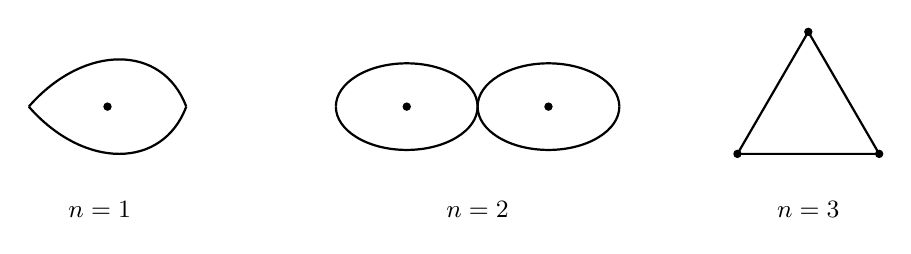
\begin{tikzpicture}[font=\small]
  \begin{scope}[xshift=-4.2cm]
    \draw[thick] (-0.9,0) .. controls (-0.2,0.8) and (0.8,0.8) .. (1.1,0);
    \draw[thick] (-0.9,0) .. controls (-0.2,-0.8) and (0.8,-0.8) .. (1.1,0);
    \filldraw (0.1,0) circle (1.3pt);
    \node at (0,-1.3) {$n=1$};
  \end{scope}
  \begin{scope}
    \draw[thick] (-1.2,0) arc (180:0:0.9 and 0.55);
    \draw[thick] (-1.2,0) arc (180:360:0.9 and 0.55);
    \draw[thick] (0.6,0) arc (180:0:0.9 and 0.55);
    \draw[thick] (0.6,0) arc (180:360:0.9 and 0.55);
    \filldraw (-0.3,0) circle (1.3pt);
    \filldraw (1.5,0) circle (1.3pt);
    \node at (0.6,-1.3) {$n=2$};
  \end{scope}
  \begin{scope}[xshift=4.8cm]
    \draw[thick] (0,0.95) -- (-0.9,-0.6) -- (0.9,-0.6) -- cycle;
    \filldraw (0,0.95) circle (1.3pt);
    \filldraw (-0.9,-0.6) circle (1.3pt);
    \filldraw (0.9,-0.6) circle (1.3pt);
    \node at (0,-1.3) {$n=3$};
  \end{scope}
\end{tikzpicture}
\end{center}

图中每个黑点都表示节点。
$n=1$ 时是一条有一个自交点的有理曲线；
$n=2$ 时是两条 $\mathbb P^1$ 在两点相交形成的“二边形”；
$n=3$ 时则是三条 $\mathbb P^1$ 拼成的三角形。
这些都是半稳定而非光滑的纤维。
\end{proof}

\begin{exercise}
\label{ex:ch07-forgetful-map-degree}
设 $(M,N)=1$。
令
\[
  f:X_0(MN)\longrightarrow X_0(N)
\]
为“遗忘 $M$-部分”的映射：
把 $(E,C_{MN})$ 送到 $(E,C_N)$，其中 $C_N=C_{MN}[N]$。
说明 $f$ 是定义在 $\Q$ 上的代数曲线态射，并计算其度数。
\end{exercise}

\begin{proof}[解答]
先说明它是代数态射。
模解释下，$X_0(MN)$ 参数化带一个阶 $MN$ 循环子群的椭圆曲线，
而把 $C_{MN}$ 换成其 $N$-torsion 部分 $C_N=C_{MN}[N]$ 是一个纯代数操作：
它只用到了有限平坦子群方案的取子群过程，
与坐标选择无关，且对基变换相容。
因此它在模问题层面就是自然变换，
于是诱导一条定义在 $\Q$ 上的代数曲线态射
\[
  f:X_0(MN)\to X_0(N).
\]

下面计算次数。
固定 $X_0(N)$ 的一个一般点 $(E,C_N)$。
由于 $(M,N)=1$，
要在其上补回一个阶 $MN$ 的循环子群 $C_{MN}$，
等价于在商曲线 $E/C_N$ 中选择一个阶 $M$ 的循环子群，
或者等价地，在 $E[M]\cong (\Z/M\Z)^2$ 中选择一个阶 $M$ 的循环子群。
所以纤维大小等于
“$(\Z/M\Z)^2$ 中阶 $M$ 的循环子群个数”。

这个个数对 $M$ 是乘法性的，
故只需先算 $M=\ell^r$ 为素数幂的情形。
在群
\[
  (\Z/\ell^r\Z)^2
\]
中，阶恰为 $\ell^r$ 的生成元个数等于所有非被 $\ell$ 整除的向量个数，
也就是
\[
  \ell^{2r}-\ell^{2r-2}.
\]
每个循环子群都有
\[
  \varphi(\ell^r)=\ell^r-\ell^{r-1}=\ell^{r-1}(\ell-1)
\]
个生成元，
故阶 $\ell^r$ 的循环子群数目为
\[
  \frac{\ell^{2r}-\ell^{2r-2}}{\ell^{r-1}(\ell-1)}
  =\ell^{r-1}(\ell+1).
\]
对一般的
\[
  M=\prod_{\ell\mid M}\ell^{r_\ell}
\]
取乘积，得到
\[
  \deg f=\psi(M)=M\prod_{\ell\mid M}\left(1+\frac1\ell\right).
\]

因此遗忘 $M$-部分的映射是一条定义在 $\Q$ 上的有限态射，
其次数为
\[
  \deg f=\psi(M)=M\prod_{\ell\mid M}\left(1+\frac1\ell\right).
\]
\end{proof}

这六题把本章主线重新压缩成了一张操作清单：
模多项式负责把解析对象写成代数方程；
Hecke 对应负责把线性算子变成曲线之间的对应；
判别式与 N\'eron $n$-gon 负责把 $\Q$ 上的几何送到模 $p$ 的世界；
而遗忘映射则提醒我们，模解释从一开始就是函子性的。
只要这四件事真正连起来，
第\ref{ch:eichler-shimura-l}章的 Eichler--Shimura 理论就不会再像“天外飞来”的公式，
而会显得顺理成章。
